%----------------------1----------------------------------------
\begin{frame}[t]{Resultados y discusión.\\\textit{Entorno de pruebas.}}
\begin{itemize}
	\item Comparar las tasas de desarrollo obtenidas con los resultados obtenidos por expertos en laboratorio.
	\item Analizar el comportamiento de la dispersión de la población.
    \item Los parámetros de configuración fueron tomados del material bibliográfico de apoyo.
    \item El periodo de simulación fue de 50 días, a temperatura constante.
    \item La dirección del viento seleccionada fue la suroeste.
    \item Se generaron aleatoriamente 1.146 larvas para 25 puntos de control.
    \end{itemize}
\end{frame}

\begin{frame}[t]{Resultados y discusión. \textit{Población inicial.}}
    \begin{center}
        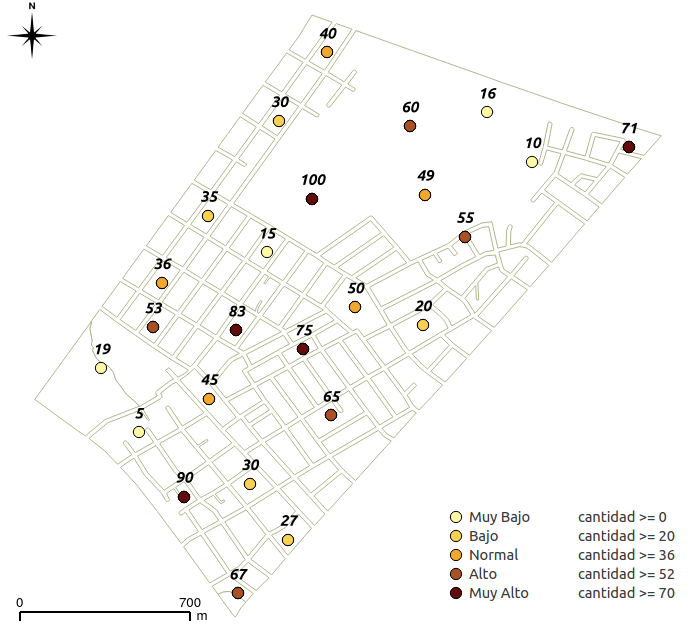
\includegraphics[width=7.5cm]{./graphics/extension-poblacion.png}
    \end{center}
\end{frame}
%--------------------------2------------------------------------
\begin{frame}[t]{Resultados y discusión.\\\textit{Tasas de desarrollo.}}
Los resultados obtenidos, fueron comparados con los valores observados en laboratorio, por Beserra, Eduardo B. et al (2006) en :
\\\text{}
\\\textit{Biologia e exigências térmicas de Aedes aegypti (L.) (Diptera: Culicidae) provenientes de quatro regiões bioclimáticas da Paraíba.}
\end{frame}

\begin{frame}[t]{Resultados y discusión.\\\textit{Tasas de desarrollo de los huevos.}}
    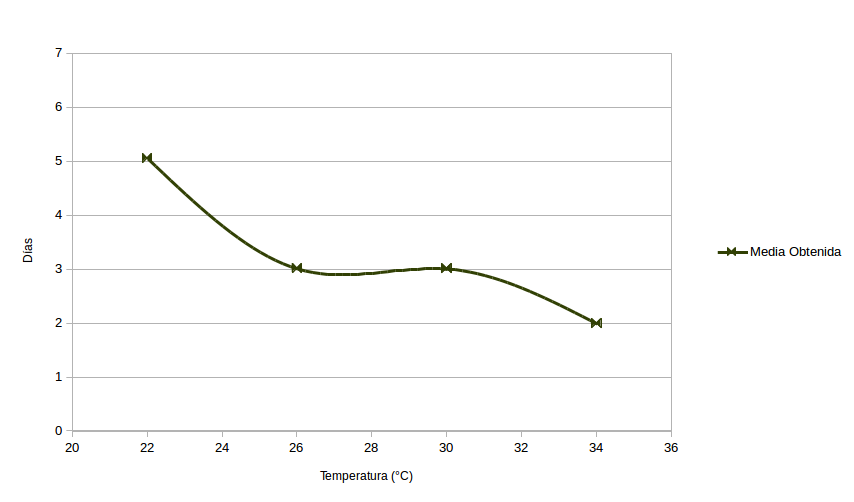
\includegraphics[width=\textwidth]{./graphics/huevos-desarrollo-single.png}
\end{frame}

\begin{frame}[t]{Resultados y discusión.\\\textit{Tasas de desarrollo de los huevos.}}
    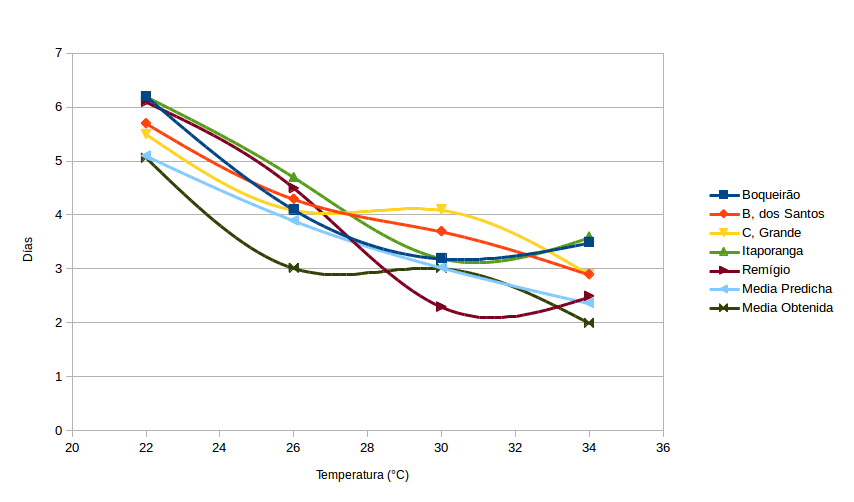
\includegraphics[width=\textwidth]{./graphics/huevos-desarrollo.png}
\end{frame}

\begin{frame}[t]{Resultados y discusión.\\\textit{Tasas de desarrollo de las larvas.}}
    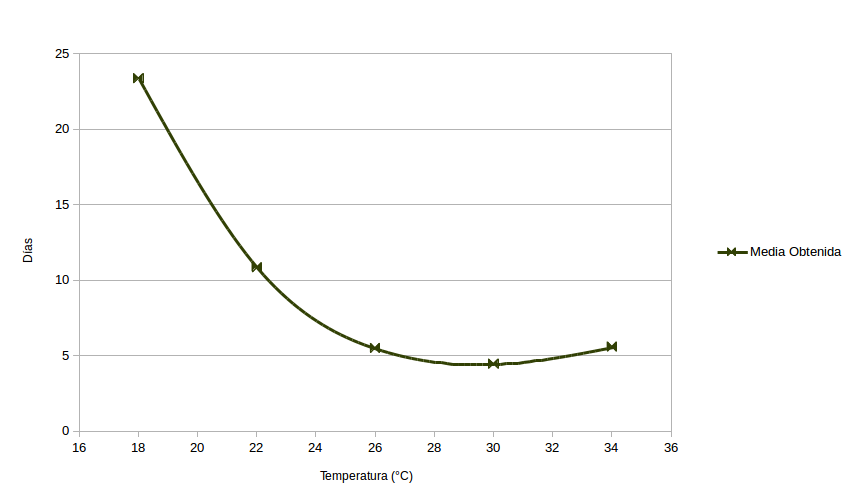
\includegraphics[width=\textwidth]{./graphics/larvas-desarrollo-single.png}
\end{frame}

\begin{frame}[t]{Resultados y discusión.\\\textit{Tasas de desarrollo de las larvas.}}
    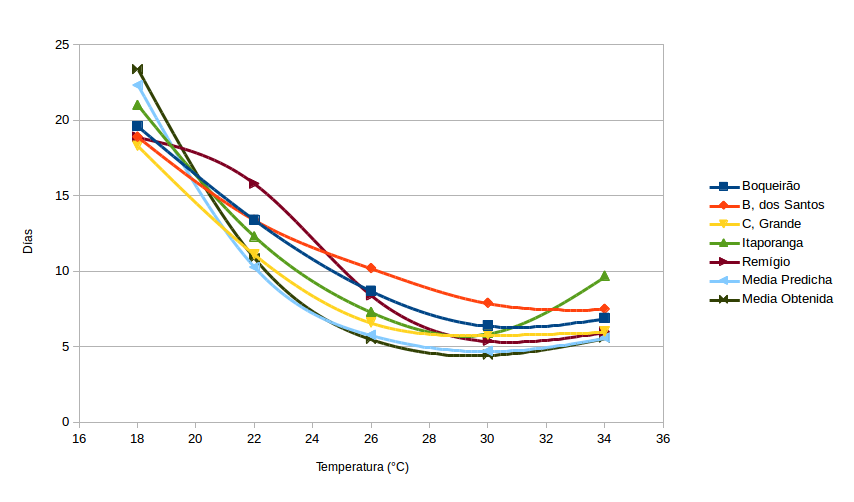
\includegraphics[width=\textwidth]{./graphics/larvas-desarrollo.png}
\end{frame}

\begin{frame}[c]{Resultados y discusión.\\\textit{Tasas de desarrollo de las pupas.}}
    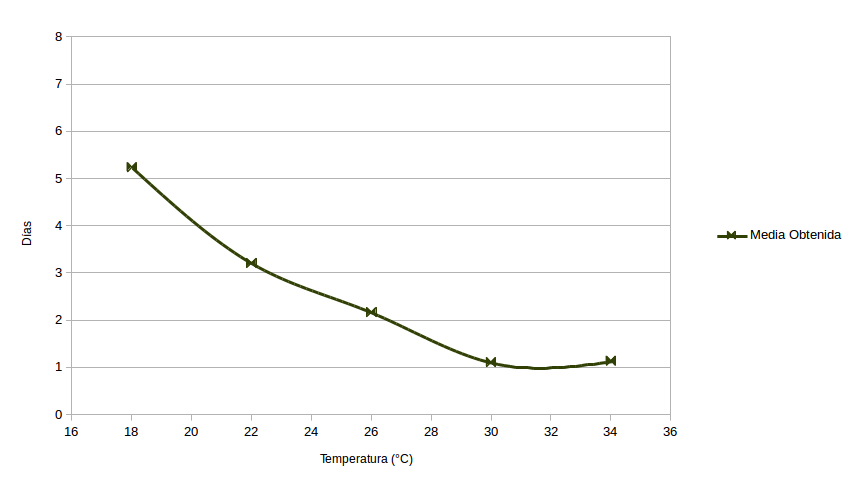
\includegraphics[width=\textwidth]{./graphics/pupas-desarrollo-single.png}
\end{frame}

\begin{frame}[c]{Resultados y discusión.\\\textit{Tasas de desarrollo de las pupas.}}
    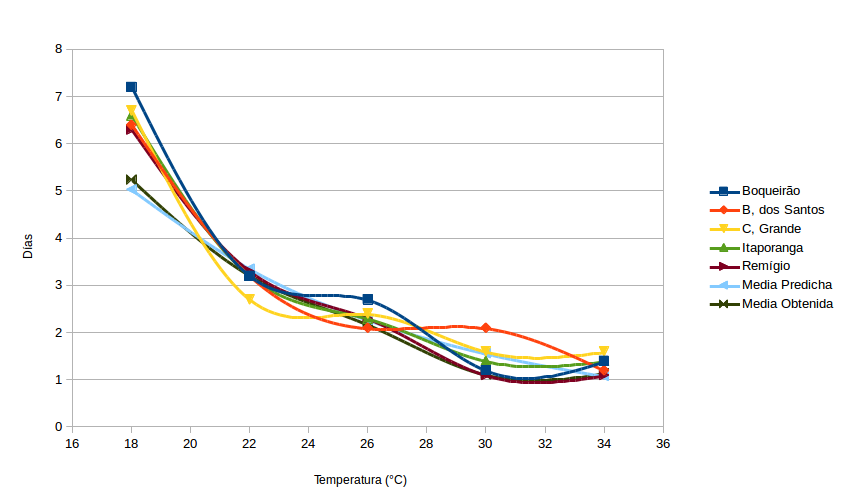
\includegraphics[width=\textwidth]{./graphics/pupas-desarrollo.png}
\end{frame}

\begin{frame}[t]{Resultados y discusión.\\\textit{Ciclo gonotrófico.}}
    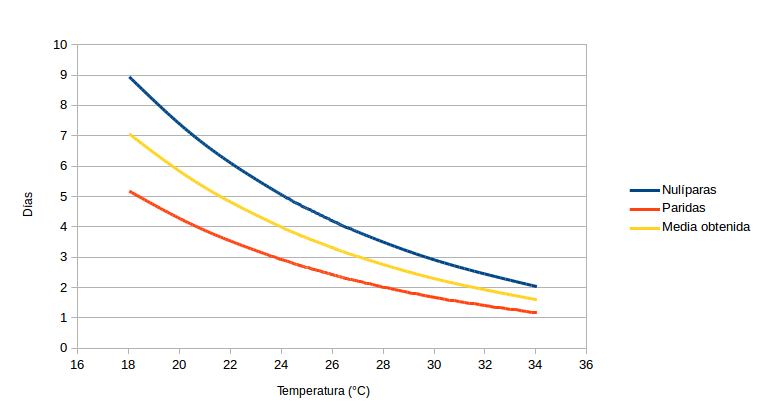
\includegraphics[width=\textwidth]{./graphics/ciclo-gonotrofico-temperatura.png}
\end{frame}

%--------------------------2------------------------------------

\begin{frame}[t]{Resultados y discusión.\\\textit{Crecimiento de la población en etapas inmaduras.}}
\begin{center}
    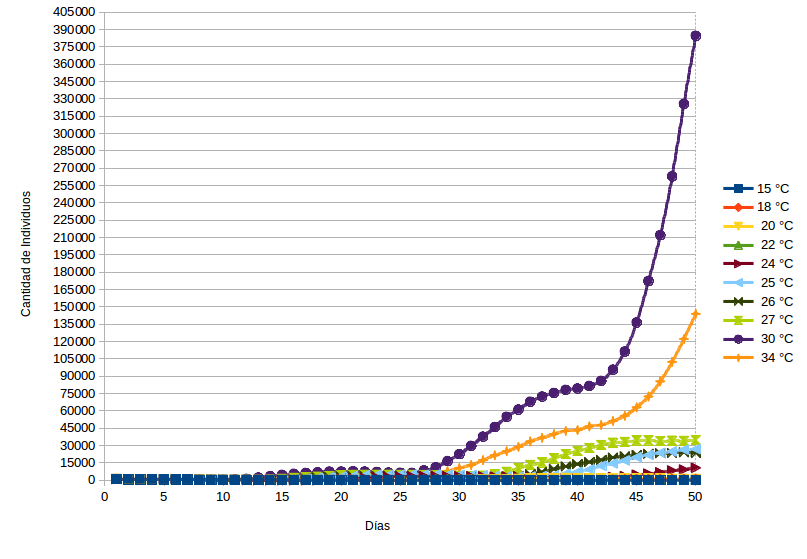
\includegraphics[width=9.3cm]{./graphics/evolucion-poblacion-all.png}
\end{center}
\end{frame}

\begin{frame}[t]{Resultados y discusión.\\\textit{Crecimiento de la población en etapas inmaduras.}}
\begin{center}
\begin{figure}
     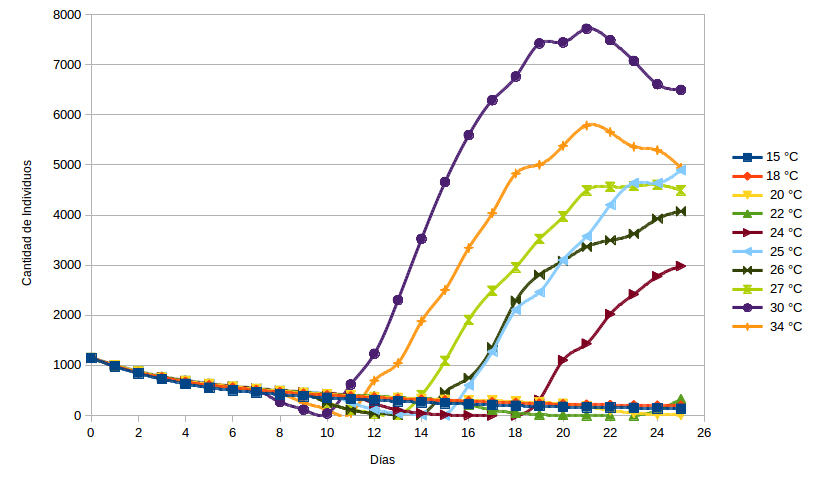
\includegraphics[width=9.3cm]{./graphics/poblacion-inmadura-p1.png}
     \caption{Del día 1 al 25.}
\end{figure}
\end{center}
\end{frame}

\begin{frame}[t]{Resultados y discusión.\\\textit{Crecimiento de la población en etapas inmaduras.}}
\begin{center}
\begin{figure}
    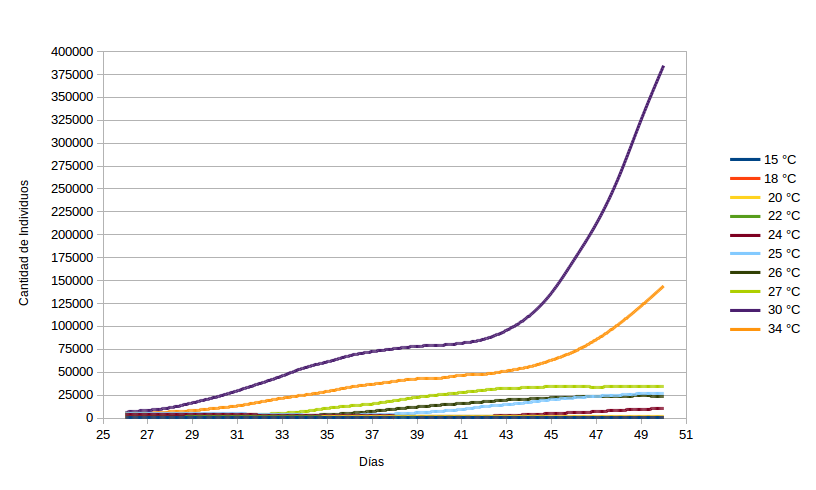
\includegraphics[width=9.3cm]{./graphics/poblacion-inmadura-p2.png}
    \caption{Del día 26 al 50.}
\end{figure}
\end{center}
\end{frame}

\begin{frame}[t]{Resultados y discusión.\\\textit{Crecimiento de la población de hembras adultas.}}
\begin{center}
    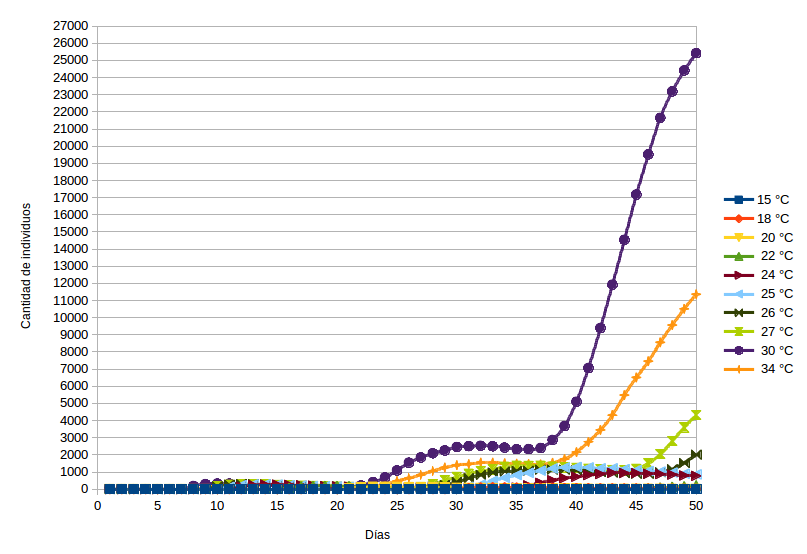
\includegraphics[width=9.3cm]{./graphics/evolucion-poblacion-adultos.png}
\end{center}
\end{frame}

\begin{frame}[t]{Resultados y discusión.\\\textit{Crecimiento de la población de hembras adultas.}}
\begin{center}
\begin{figure}
    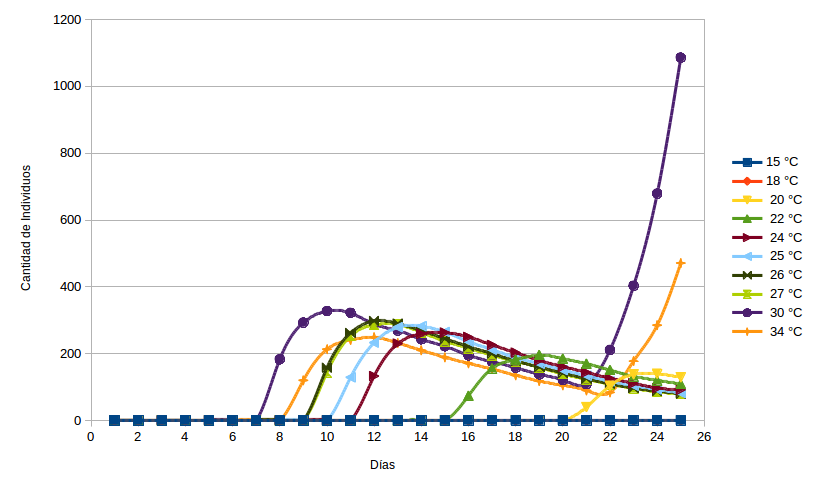
\includegraphics[width=9.3cm]{./graphics/poblacion-adulto-p1.png}
    \caption{Del día 1 al 25.}
\end{figure}
\end{center}
\end{frame}

\begin{frame}[t]{Resultados y discusión.\\\textit{Crecimiento de la población de hembras adultas.}}
\begin{figure}
    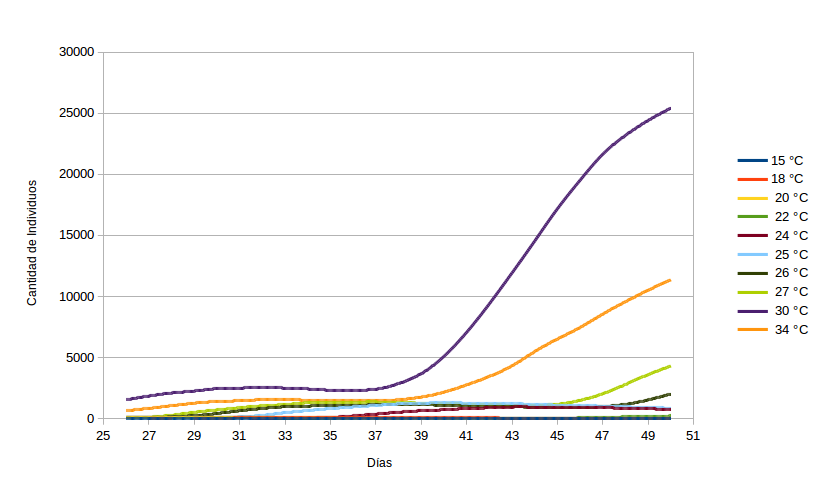
\includegraphics[width=9.3cm]{./graphics/poblacion-adulto-p2.png}
    \caption{Del día 26 al 50.}
\end{figure}
\end{frame}

\begin{frame}[t]{Resultados y discusión.\\\textit{Análisis espacial de la población.}}
\begin{center}
    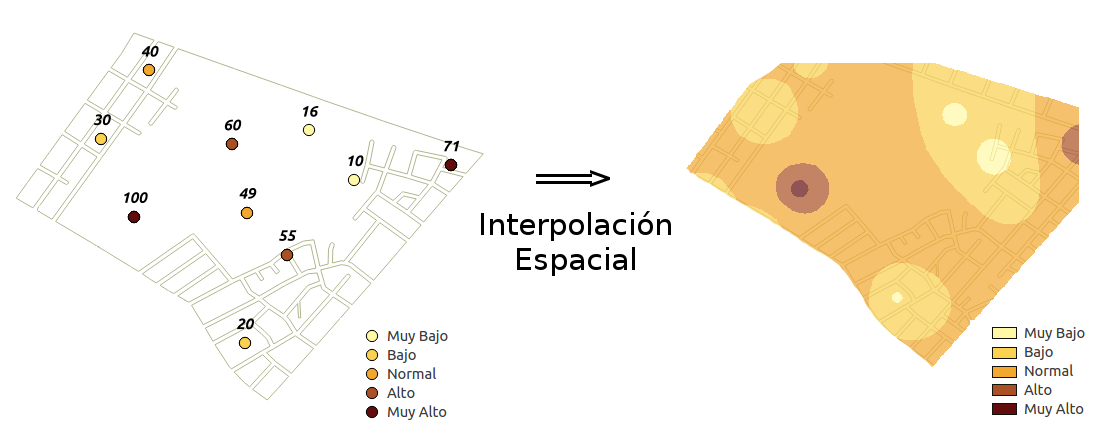
\includegraphics[width=11cm]{./graphics/identificacion-focos.png}
\end{center}
\end{frame}

\begin{frame}[t]{Resultados y discusión.\\\textit{Mapas de interpolación.}}
\begin{center}
    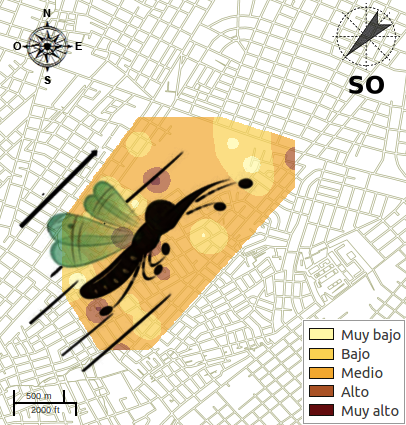
\includegraphics[width=5cm]{./graphics/raster-dispersion.png}
\end{center}
\end{frame}

\begin{frame}[t]{Resultados y discusión.\\\textit{Mapas de interpolación a 30 \textcelsius.}}
    \begin{figure}
    \begin{subfigure}[b]{0.45\textwidth}
        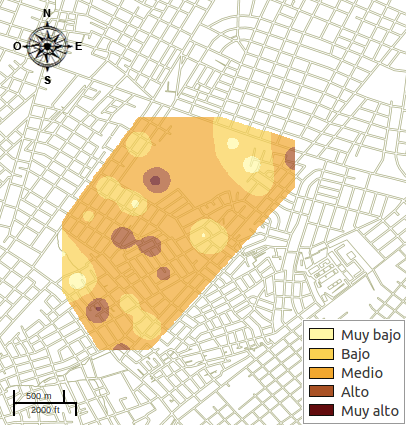
\includegraphics[width=\textwidth]{../book/capitulo-6/graphics/raster/temp-30-0.png}
        \caption{Primer día de simulación.}
    \end{subfigure}
    ~~~~
    \begin{subfigure}[b]{0.45\textwidth}
        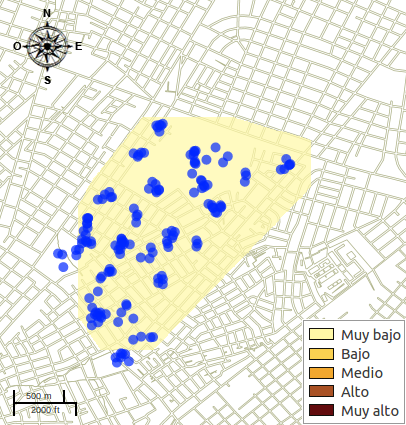
\includegraphics[width=\textwidth]{../book/capitulo-6/graphics/raster/temp-30-9.png}
        \caption{Día número 10 de simulación.}
    \end{subfigure}
    \end{figure}
\end{frame}


\begin{frame}[t]{Resultados y discusión.\\\textit{Mapas de interpolación a 30 \textcelsius.}}
    \begin{figure}
    \begin{subfigure}[b]{0.45\textwidth}
        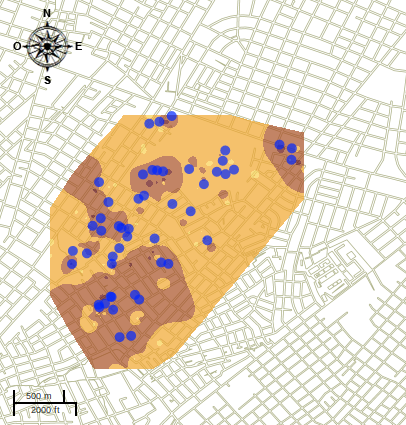
\includegraphics[width=\textwidth]{../book/capitulo-6/graphics/raster/temp-30-20.png}
        \caption{Día número 21 de simulación.}
    \end{subfigure}
    ~~~~
    \begin{subfigure}[b]{0.45\textwidth}
        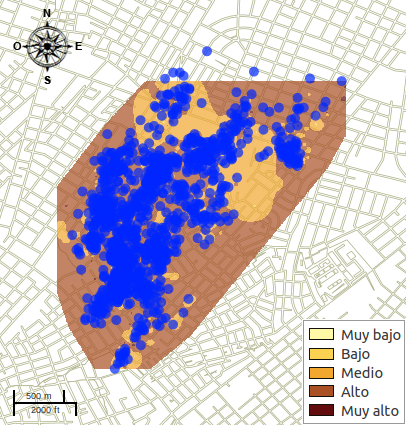
\includegraphics[width=\textwidth]{../book/capitulo-6/graphics/raster/temp-30-35.png}
        \caption{Día número 50 de simulación.}
    \end{subfigure}
    \end{figure}
\end{frame}

\begin{frame}[t]{Resultados y discusión.\\\textit{Mapas de interpolación a 30 \textcelsius.}}
    \begin{figure}
    \begin{subfigure}[b]{0.45\textwidth}
        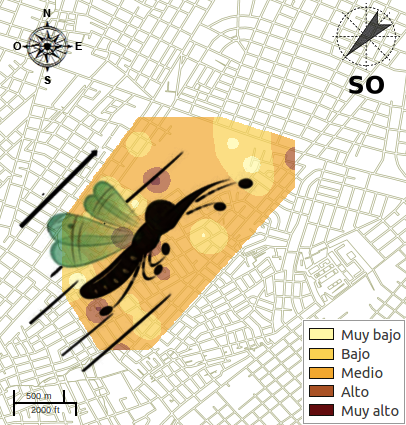
\includegraphics[width=\textwidth]{./graphics/raster-dispersion.png}
        \caption{Primer día de simulación.}
    \end{subfigure}
    ~~~~
    \begin{subfigure}[b]{0.45\textwidth}
        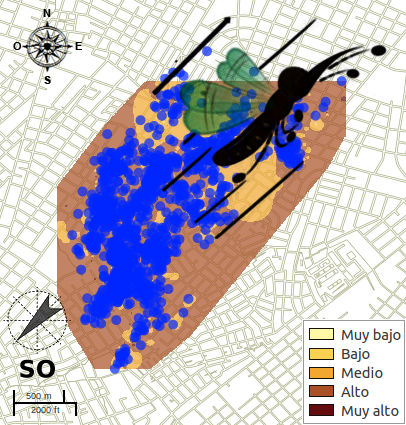
\includegraphics[width=\textwidth]{./graphics/raster-dispersion-final.png}
        \caption{Día número 50 de simulación.}
    \end{subfigure}
    \end{figure}
\end{frame}


\begin{frame}[t]{Resultados y discusión.\\\textit{Análisis a temperaturas variables.}}
\begin{itemize}
    \item Temperaturas variables correspondientes al año 2010.
    \item Datos pertenecientes a la ciudad de Villarrica (enero-diciembre).
    \item Periodo de simulación igual a 365 días.
    \item Temperatura media anual de 21,67 \textcelsius.
    \end{itemize}
\end{frame}

\begin{frame}[t]{Resultados y discusión.\\\textit{Análisis a temperaturas variables.}}
    \begin{figure}
    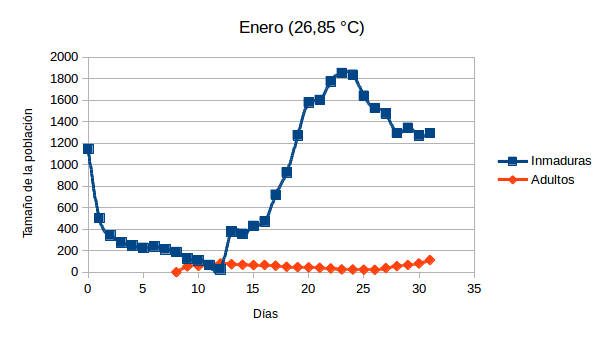
\includegraphics[width=\textwidth]{./graphics/py-2010-enero.png}
    \end{figure}
\end{frame}

\begin{frame}[t]{Resultados y discusión.\\\textit{Análisis a temperaturas variables.}}
    \begin{figure}
    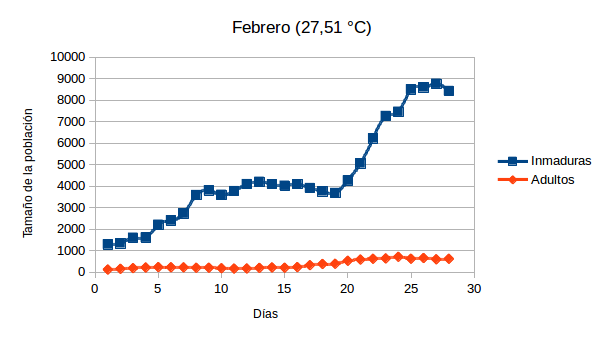
\includegraphics[width=\textwidth]{./graphics/py-2010-febrero.png}
    \end{figure}
\end{frame}

\begin{frame}[t]{Resultados y discusión.\\\textit{Análisis a temperaturas variables.}}
    \begin{figure}
    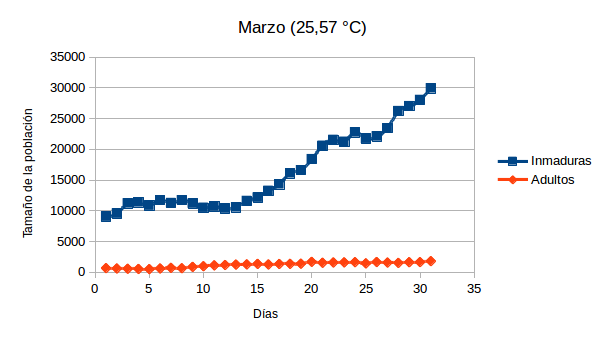
\includegraphics[width=\textwidth]{./graphics/py-2010-marzo.png}
    \end{figure}
\end{frame}

\begin{frame}[t]{Resultados y discusión.\\\textit{Análisis a temperaturas variables.}}
    \begin{figure}
    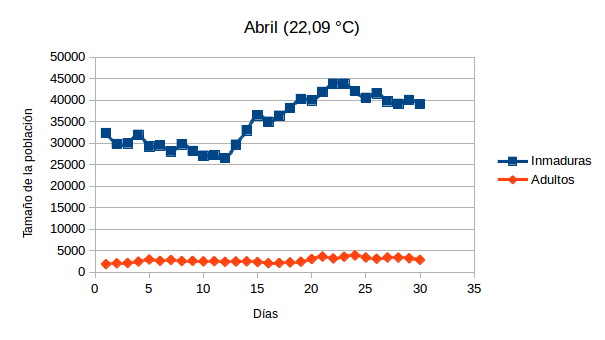
\includegraphics[width=\textwidth]{./graphics/py-2010-abril.png}
    \end{figure}
\end{frame}


\begin{frame}[t]{Resultados y discusión.\\\textit{Análisis a temperaturas variables.}}
    \begin{figure}
    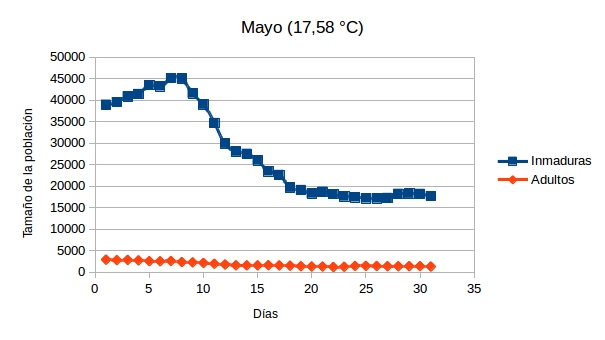
\includegraphics[width=\textwidth]{./graphics/py-2010-mayo.png}
    \end{figure}
\end{frame}

\begin{frame}[t]{Resultados y discusión.\\\textit{Análisis a temperaturas variables.}}
    \begin{figure}
    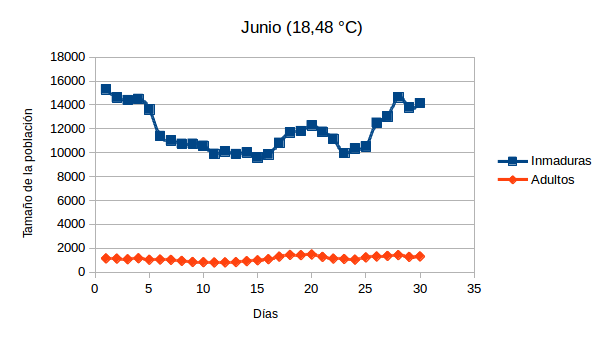
\includegraphics[width=\textwidth]{./graphics/py-2010-junio.png}
    \end{figure}
\end{frame}

\begin{frame}[t]{Resultados y discusión.\\\textit{Análisis a temperaturas variables.}}
    \begin{figure}
    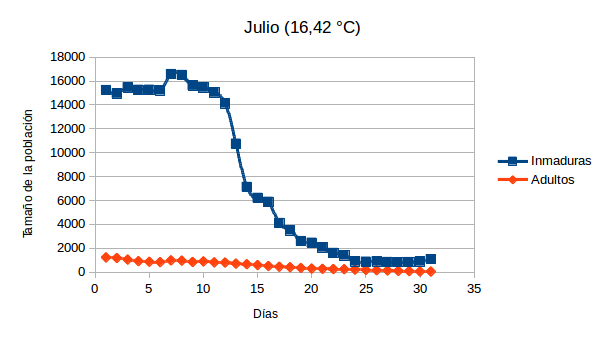
\includegraphics[width=\textwidth]{./graphics/py-2010-julio.png}
    \end{figure}
\end{frame}

\begin{frame}[t]{Resultados y discusión.\\\textit{Análisis a temperaturas variables.}}
    \begin{figure}
    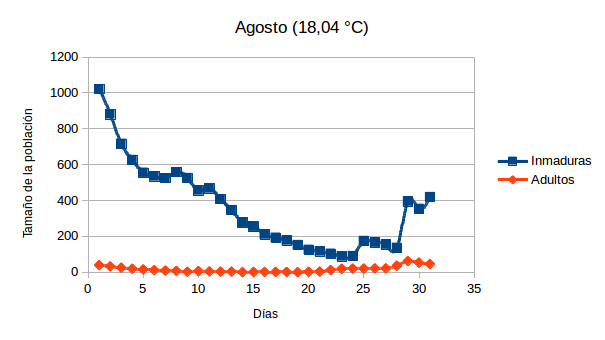
\includegraphics[width=\textwidth]{./graphics/py-2010-agosto.png}
    \end{figure}
\end{frame}

\begin{frame}[t]{Resultados y discusión.\\\textit{Análisis a temperaturas variables.}}
    \begin{figure}
    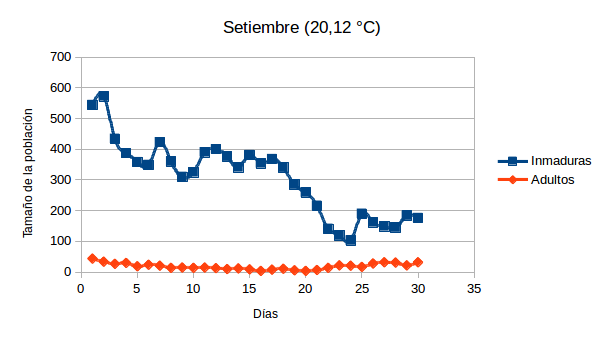
\includegraphics[width=\textwidth]{./graphics/py-2010-septiembre.png}
    \end{figure}
\end{frame}

\begin{frame}[t]{Resultados y discusión.\\\textit{Análisis a temperaturas variables.}}
    \begin{figure}
    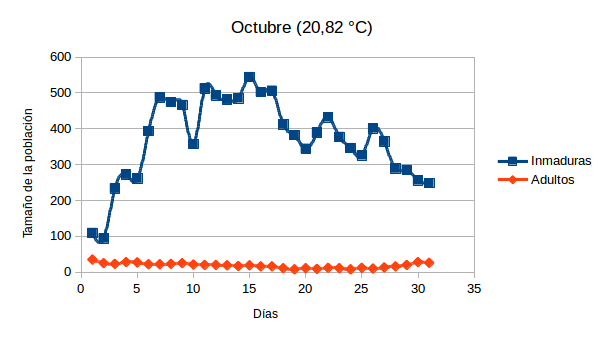
\includegraphics[width=\textwidth]{./graphics/py-2010-octubre.png}
    \end{figure}
\end{frame}

\begin{frame}[t]{Resultados y discusión.\\\textit{Análisis a temperaturas variables.}}
    \begin{figure}
    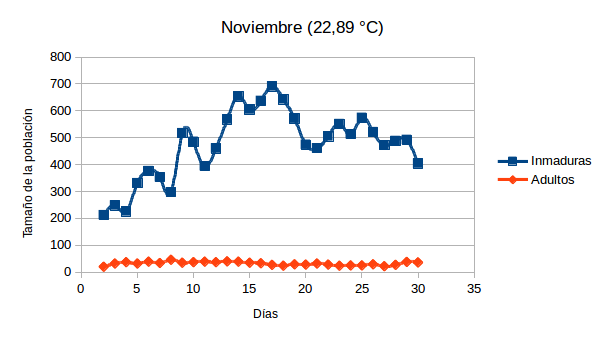
\includegraphics[width=\textwidth]{./graphics/py-2010-noviembre.png}
    \end{figure}
\end{frame}

\begin{frame}[t]{Resultados y discusión.\\\textit{Análisis a temperaturas variables.}}
    \begin{figure}
    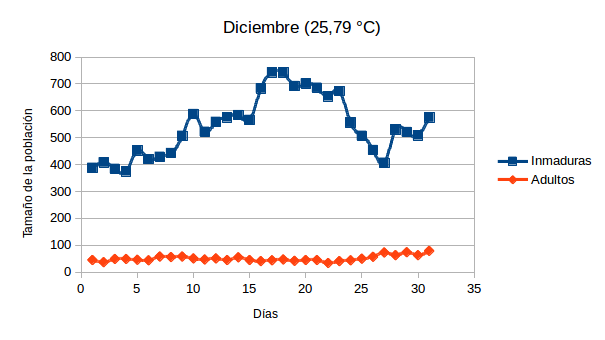
\includegraphics[width=\textwidth]{./graphics/py-2010-diciembre.png}
    \end{figure}
\end{frame}
